% To je predloga za poročila o domačih nalogah pri predmetih, katerih
% nosilec je Tomaž Curk. Avtor predloge je Blaž Zupan.
%
% Seveda lahko tudi dodaš kakšen nov, zanimiv in uporaben element, 
% ki ga v tej predlogi (še) ni. Več o LaTeX-u izveš na
% spletu, na primer na http://tobi.oetiker.ch/lshort/lshort.pdf.
%
% To predlogo lahko spremeniš v PDF dokument s pomočjo programa
% pdflatex, ki je del standardne instalacije LaTeX programov.

\documentclass[a4paper,11pt]{article}
\usepackage{a4wide}
\usepackage{fullpage}
\usepackage[utf8x]{inputenc}
\usepackage[slovene]{babel}
\selectlanguage{slovene}
\usepackage[toc,page]{appendix}
\usepackage[pdftex]{graphicx} % za slike
\usepackage{setspace}
\usepackage{color}
\definecolor{light-gray}{gray}{0.95}
\usepackage{listings} % za vključevanje kode
\usepackage{hyperref}
\renewcommand{\baselinestretch}{1.2} % za boljšo berljivost večji razmak
\renewcommand{\appendixpagename}{Priloge}

\lstset{ % nastavitve za izpis kode, sem lahko tudi kaj dodaš/spremeniš
language=Python,
basicstyle=\footnotesize,
basicstyle=\ttfamily\footnotesize\setstretch{1},
backgroundcolor=\color{light-gray},
}

\title{Nenadzorovano modeliranje}
\author{Primož Pečar (63150213)}
\date{\today}

\begin{document}

\maketitle

\section{Uvod}

V drugi domači nalogi sem se ukvarjal z iskanjem osamelcev in gručenjem sorodnih primerov na podatkovni množici Movie Lens.

\section{Podatki}

Večina podatkov je bilo kopiranih iz prve domače naloge, saj sem tam imel že vse pripravljeno. Kar je na novo je xlsx datoteka, ki je bila posebaj pripravljena za uporabo z Orange3.


\section{Metode}

Prva naloga in podnaloge so popolnoma rešene v Pythonu, pri drugi nalogi pa so podatki pripravljeni za uporabo z Orange3, saj sem tam lahko hitreje testiral različne metode hierarhičnega gručenja, potreben je bil le pravilen format xlsx datoteke.


\section{Naloge podrobno}

V tem odseku bom opisal vsako od nalog bolj podrobno. Govoril bom o ugotovitvah, do katerih sem prišel med nalogo in zanimivostih, ki sem jih srečal.

\subsection{Naloga 1}

V prvi nalogi je bilo potrebno ugotoviti, ocene katerih filmov so najbolj enotne. Zanimalo nas je, če obstajajo filmi, ki so dobili podobne ocene med vsemi uporabniki ali pa filmi z razpršenimi ocenami.

\subsubsection{Ustrezna naključna spremenljivka}


Potrebno je bilo ugotoviti, s katerimi podatki si lahko pomagamo pri ugotavljanju povezav med filmi. Spremenljivka, ki sem jo uporabil so bili ratingi. Za vsak film posebaj sem izračunal standardni odklon in nato vse filme predstavil v histogramu.

\subsubsection{Porazdelitev}

Porazdelitev se je spreminjala na podlagi parametrov filmov. Kot v prvi nalogi sem upošteval filme, ki imajo 30 ali več ocen, tako se znebim filmov, ki imajo po eno ali celo nič ocen in robnih primerov, kot so naprimer neznani filmi. Porazdelitev, ki sem jo dobil je bila normalna. Saj je 68\% primerov v prvem odklonu (na sredini), potem 95\% v drugem odklonu in 99.7\% v tretjem. V primeru, da sem upošteval vse filme, pa sem dobil Beta porazdelitev.
\begin{figure}[htbp]
	\begin{center}
		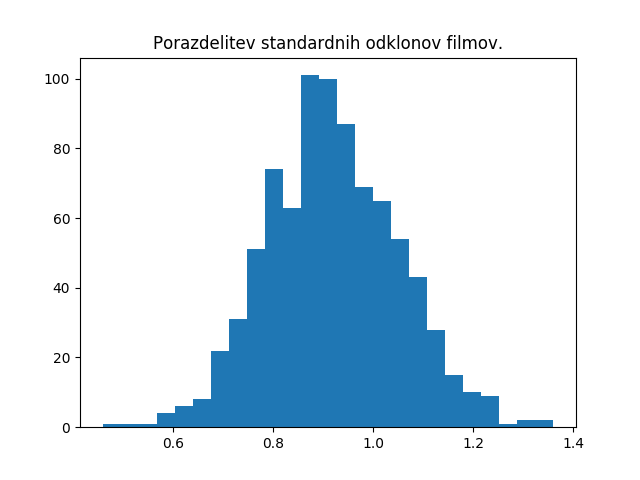
\includegraphics[scale=0.6]{../slike/std_movie.png}
		\caption{Histogram standardnih odklonov filmov.}
		\label{zanri_slika}
	\end{center}
\end{figure}
\pagebreak

\subsubsection{Ocena parametrov}
Za oceno parametrov sem uporabil sledeče formule:

$\mu = E[X_i] = \bar{X}$   (povprečje vzorca)

$\sigma^2 = \frac{n-1}{n} E[(X_i-\bar{X})^2] = \frac{n-1}{n} var[x]$ (popravljena varianca vzorca)

V kodo se prevede sledeče, kjer je mySTD seznam vseh standardnih odklonov filmov:

\begin{lstlisting}[frame=single]  % Start your code-block

mu_fit = np.mean(mySTD)
n = len(mySTD)
sigma2_fit = (n-1)/n * np.var(mySTD)
print("##########OCENA###########")
print(mu_fit,sigma2_fit)
\end{lstlisting}
Dobil sem kar dobro oceno, predvidevam zaradi tega ker sem uporabil le filme, ki imajo 30 ali več ocen. (Prva številka je povprečje vzorca, druga pa popravljena varianca vzorca.)
\textbf{0.919678380176 0.017390364507}

\subsubsection{Izbira porazdelitve}
Kot omenjeno, porazdelitev je zelo verjetno normalna, saj ima zvonasto obliko, po kateri je znana. Na vajah pa smo spoznali še studentovo, beta, normalno oz. gaussovo porazdelitev. Razvedrilo za bralca, poskušal sem izrisati ocenjeno in resnično porazdelitev, vendar je rezultat bil sledeč.
\begin{figure}[htbp]
	\begin{center}
		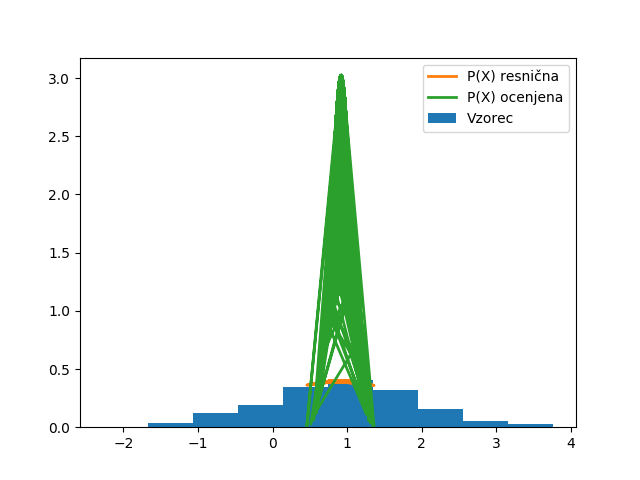
\includegraphics[scale=0.6]{../slike/i_tried.png}
		\caption{Skoraj normalna porazdelitev.}
		\label{zanri_slika}
	\end{center}
\end{figure}
\pagebreak


\subsubsection{Zgornjih 5\% }
Tukaj pa sem gledal primere, ki so v tretjem odklonu, torej vse filme, ki so manjši od 0.6 in večji od 1.2. Tako dobimo tiste res edinstvene filme, ki so v povprečju zelo slabo ocenjeni s strani gledalcev in tiste, ki so zelo dobro ocenjeni.
\begin{table}[htbp]
	\caption{Padajočih 5\%}
	\label{tab_pad}
	\begin{center}
		\begin{tabular}{llp{3cm}}
			
			\hline
			Ime filma & Standardni odklon \\
			\hline
			Roger \& Me (1989) & 0.582847222138 \\
			Blood Diamond (2006) & 0.511732330507\\  
			Deliverance (1972) & 0.596212000886\\
			Harry Potter and the Deathly Hallows: Part 2 (2011) & 0.596449993843\\
			Scent of a Woman (1992) & 0.553022000768\\
			Muppet Movie & 0.459813626841 \\
			Delicatessen (1991) & 0.596284794\\
			\hline
		\end{tabular}
	\end{center}
\end{table}

\begin{table}[htbp]
	\caption{Naraščajočih 5\%}
	\label{tab_pad}
	\begin{center}
		\begin{tabular}{llp{3cm}}
			
			\hline
			Ime filma & Standardni odklon \\
			\hline
			Mad Max: Fury Road (2015) & 1.3426874444 \\
			Star Wars: Episode II - Attack of the Clones (2002) & 1.25118920231\\
			Space Jam (1996) & 1.22784363825 \\
			Saw (2004) & 1.36009641532 \\
			Blair Witch Project & 1.31123664377 \\
			Showgirls (1995) & 1.259737582 \\
			\hline
		\end{tabular}
	\end{center}
\end{table}

\subsection{Naloga 2}
V drugi nalogi je bilo potrebno poiskati 100 najbolj gledanih filmov. Vzel sem vse filme in jih sortiral padajoče po ogledih in vzel vrhnjih 100. Potrebno je bilo narediti vektor, po imenu filma, atributi so bili pa vsi uporabniki. Tako smo dobili matriko, katera je imela ratinge vseh uporabnikov za vsak film, če uporabnik ni ocenil filma sem tam zapisal ?.


\begin{table}[htbp]
	\caption{Padajoče ocenjeni filmi}
	\label{tab_pad}
	\begin{center}
		\begin{tabular}{llp{3cm}}
			
			\hline
			Forrest Gump (1994) 						& 4.054252 & 341 \\
			Pulp Fiction (1994)		   					& 4.487138 & 324 \\  
			The Shawshank Redemption (1994)				& 4.487138 & 311 \\
           	Silence of the Lambs, The (1991)			& 4.138157 & 304 \\
			Star Wars: Episode IV - A New Hope (1977)	& 4.221649 & 291 \\
			\hline
		\end{tabular}
	\end{center}
\end{table}

\begin{table}[htbp]
	\caption{Naraščujoče ocenjeni filmi}
	\label{tab_nar}
	\begin{center}
		\begin{tabular}{llp{3cm}}
			\hline
			Ime filma & Povprečen rating & Število ocen \\
			\hline
			Dune (1984)			 				& 3.0833333  	& 30 \\
			National Lampoon's Vacation (1983)  & 3.6833333 	& 30 \\  
			Panic Room (2002)					& 3.2166666 	& 30 \\
			The Bone Collector (1999)			&2.88333333 	& 30 \\
			The Jungle Book (1994)				& 4.221649 		& 30 \\
			\hline
		\end{tabular}
	\end{center}
\end{table}
\pagebreak

\subsection{Naloga 4}
V četrti nalogi smo morali preveriti povezanost med timestampom ter povprečno oceno filma za tisti časovni odsek. V python kodi sem naredil primere za 4 filme, 2 najbolje ocenjena (Godfather, Shawshank Redemption) in 2 narslabše ocenjena (Home Alone,Charlie's angels). Preverjal sem kako se je za nek zelo dober filem čez čas spreminjala ocena, ter kako za nek slab film. Ugotovil sem, da ocena bolj ali manj kroži okoli splošnega povprečja filma.

\begin{figure}[htbp]
		\begin{center}
		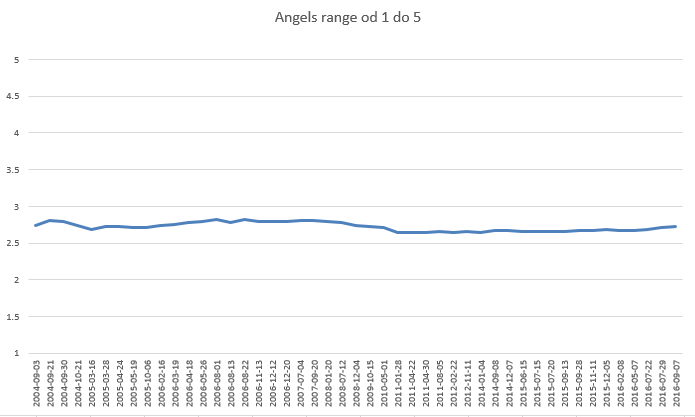
\includegraphics[scale=0.8]{../slike/agnels_range.png}
		\caption{Porazdelitev Angelov}
		\label{angeli_range}
		\end{center}
\end{figure}


\begin{figure}[htbp]
	\begin{center}
		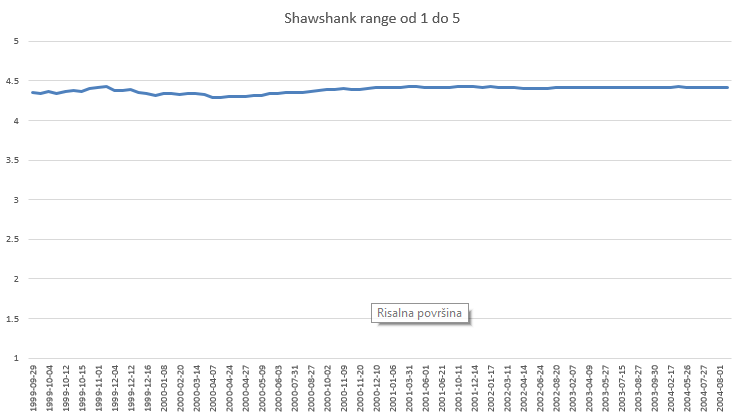
\includegraphics[scale=0.8]{../slike/shawshank_range.png}
		\caption{Porazdelitev Shawshank}
		\label{shawk_range}
	\end{center}
\end{figure}

\begin{figure}[htbp]
	\begin{center}
		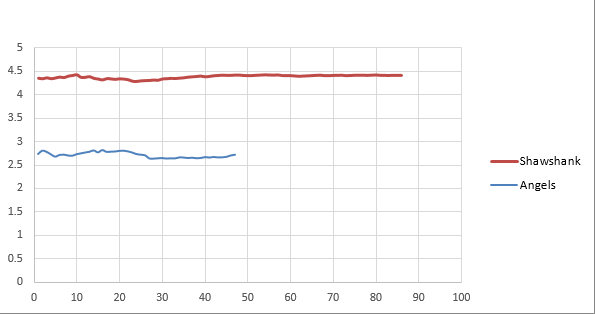
\includegraphics[scale=0.9]{../slike/skupno_ocene.png}
		\caption{Ponazorjen primer povprečnih ocen zgornjih filmov, glede na št. ocen}
		\label{skupno_range}
	\end{center}
\end{figure}
\pagebreak
 
\subsection{Naloga 5}
V peti nalogi smo morali ugotoviti, kateri so najbolj popularni igralci. Vzel sem 500 najbolj ocenjenih filmov in pogledal kateri igralci so igrali v teh filmih. To sem združil v slovar kjer je key igralec, vrednost pa št. pojavitev v igranih filmih. Potem sem vzel slovar, ga sortiral padajoče in izpisal prvih 10 igralcev, to pa sem vizualiziral v histogramu. 

\begin{figure}[htbp]
	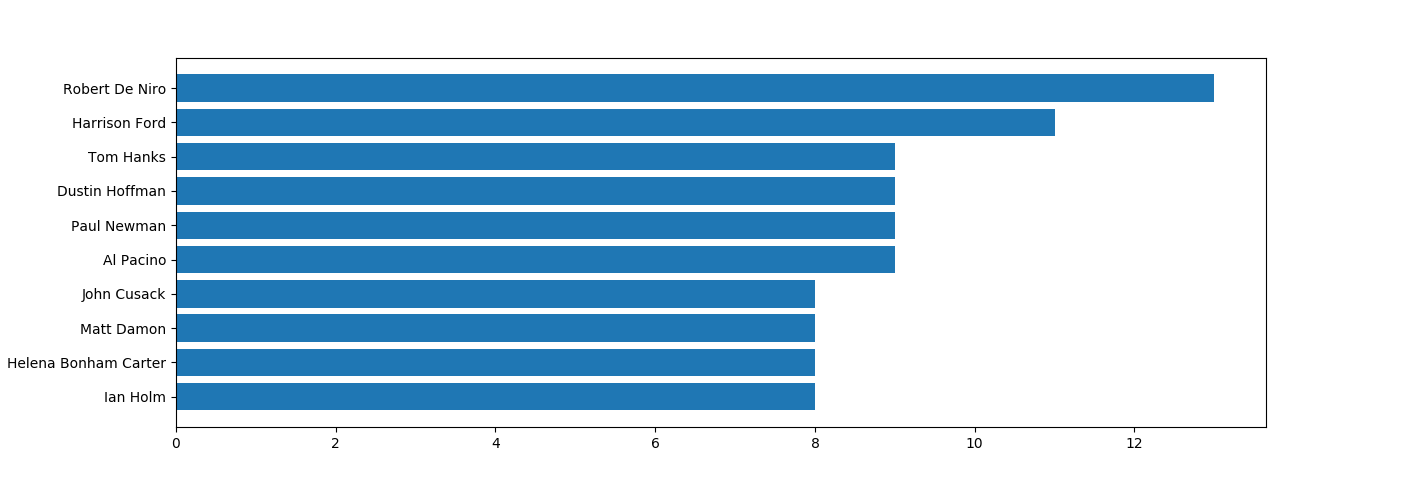
\includegraphics[scale=0.55]{../slike/pop_actors.png}
	\caption{Ponazorjen primer povprečnih ocen zgornjih filmov, glede na št. ocen}
	\label{pop_act}
\end{figure}


\subsection{Naloga 6}
The Grand Budapest Hotel, nevem kaj je s tem filmom, ampak način kako je bila zgodba prikazana, in da se film ne jemlje preveč resno mi je bil zelo všeč.
\pagebreak


\section{Rezultati}

Tukaj pa so bolj posplošeni rezultati za vsako od nalog.
  Prva naloga enačimo movieID od ratinov in moviev, združimo ratinge in imena filmov in izpišemo v padajočem vrstnem redu.
  
  Duga naloga samo splittamo žanre in povečujemo nek counter, vsakič ko se pojavi določen žanr.
  
  Tretja naloga gledamo najmanj in najbolj gledane filme in njihove povprečne ocene, ugotovimo, da so filmi bolj ali manj nagnjeni k povprečju, brez nekih hudih izjem.
  
  Četrta naloga vzamemo rating in datum ko je bil ocenjen, spremljamo kako se spreminja povprečje od začetka do "konca". Ugotovimo, da že od začetka dobro ocenjeni filmi ostanejo z dobrim povprečjem in obratno za slabe.
  
  Peta naloga pa vzamemo 500 najboljših filmov in iz actors jemljemo igralce, povečujemo counter, za vsakega izmed igralcev in na koncu izpišemo 10 najpopularnejših igralcev.
  

\section{Izjava o izdelavi domače naloge}
Domačo nalogo in pripadajoče programe sem izdelal sam.

\appendix
\appendixpage
\section{\label{app-res}Slike in programska koda}

Slike se nahajajo v mapi slike, programska koda v source, LaTex datoteke pa v tex.



\end{document}
